\chapter{Evaluation}
\label{Evaluation}
\textit{This chapter describes the evaluation of WebTaint. The chapter starts with a description of the \textit{\nameref{TestEnvironment}} followed by a detailed description of the \textit{\nameref{Benchmarking}}.}



\section{Test Environment}
\label{TestEnvironment}
The benchmarks are conducted on an Asus Zenbook UZ32LN, bought in spring 2015. No other programs were running while benchmarks were in process. The specifications of the computer and other important metrics are the following:

\begin{description}
    \item [Processor:] 2 GHz i7-4510U
    \item [Memory:] 8 GB 1600 MHz DDR3
    \item [Operating system:] Ubuntu 17.10
    \item [Java:] OpenJDK 1.8.0\_162
    \item [Java Virtual Machine:] OpenJDK 25.162-b12, 64-Bit, mixed mode
\end{description}



\section{Benchmarking}
\label{Benchmarking}
The benchmarks conducted are on applications, where we will look at security gain, and on a performance benchmarking suit where time and memory overhead was examined. To evaluate the security gain and performance overhead is every benchmark executed twice. The first time is without WebTaint activated and the second with WebTaint activated. The reason behind this is first to acquire the baseline values which then can be used to compare with the WebTaint values. The difference between these is the security gain and performance overhead.



\subsection{Applications}
To detect security vulnerabilities in the applications has OWASP Zed Attack Proxy \parencite{zap} known as ZAP ben used. ZAP is an open-source security scanner for web applications which is widely used in the penetration testing industry. Usage of ZAP is seen in Figure \ref{fig:ZAP}. ZAP accesses the web application over HTTP(S) communication and tries to find vulnerabilities in the applications wherever user input is possible.

\begin{figure}[H]
    \centering
    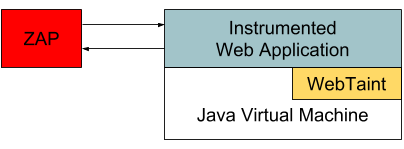
\includegraphics[width=0.8\textwidth]{images/ZAPArchitecture.png}
    \caption{Evaluation architecture of ZAP and WebTaint}
    \label{fig:ZAP}
\end{figure}

Extensive ZAP scans are very time-consuming, and to the only scan, the applications for vulnerabilities of interest is a new policy specified in ZAP. The policy is modified only to contain the Injection category where the tests in Table \ref{table:ZapTests} are used.

\begin{table}[H]
  \centering
  \caption{Security Vulnerabilities Detected by dynamic taint tracker (DTT) in Ticketbook}
    \label{table:ZapTests}
    \begin{itemize}
        \item Buffer Overflow
        \item CRLF Injection
        \item Cross-Site Scripting (Persistent)
        \item Cross-Site Scripting (Persistent) - Prime
        \item Cross-Site Scripting (Persistent) - Spider
        \item Cross-Site Scripting (Reflected)
        \item Format String Error
        \item Parameter Tampering
        \item Remote OS Command Injection
        \item SQL Injection
    \end{itemize}
\end{table}

Every scan of an application starts with spidering to detects all possible entries to the system. If the application requires authentication to access parts of the application is the needed credentials added to the ZAP context, and then execute the spider the application once again. After these steps are the scanning of the application started and possible vulnerabilities found are stored in log files.

The benchmarking of applications are a very time-consuming task and therefore only conducted on four applications. Each application is Java-based, and all of them are containing security vulnerabilities including one or more of SQL Injection attacks or Cross-Site Scripting. These four Java web applications are presented in the sections below.



\subsubsection{Stanford SecuriBench Micro}
Stanford SecuriBench Micro is a set of small test cases designed to evaluate security analyzers. The test suit deliberately insecure and was created as part of the Griffin Security Project \parencite{griffin} at Stanford University and contains 96 test cases and 46407 lines of code. This thesis uses version 1.08 of the application and contains the vulnerabilities SQL Injection, Cross-Site Scripting, HTTP Splitting, Path Traversal and more \parencite{securiBenchMicro, microfaq}. 



\subsubsection{InsecureWebApp}
InsecureWebApp is a deliberately insecure web application developed by OWASP to show possible security vulnerabilities and what harm they can cause to a web application. The project consists of 2913 lines of code and version 1.0 is used and contains the vulnerabilities Parameter Tampering, Broken Authentication, SQL Injection, HTML Injection and more \parencite{insecure}. 



\subsubsection{Ticketbook}
Ticketbook is deliberately insecure web application developed by Contrast Security to show the power of one of their security tools. The application consist of 13849 lines of code and version 0.9.1-SNAPSHOT is used and contains the vulnerabilities Cross-Site Scripting, Command Injection, Parameter Tampering, XML External Entity and more \parencite{ticketbook, contrast}



\subsubsection{SnipSnap}
SnipSnap is a Java-based web application developed to provide the necessary infrastructure to create a collaborative encyclopedia. The web page functionality is similar to Wikipedia \parencite{wikipedia} where users can sign up and contribute by writing posts. The application consists of 566173 lines of code and version 1.0-BETA-1 is used in this thesis \parencite{snipsnap}. The application is not deliberately insecure, and the policies which it aims to fulfill is the same as specified in Subsection \ref{Integrity} and \ref{Confidentiality}. Which is to prevent unauthorized information access, and execution of code as well as preventing information disclosure.



\subsection{Performance Overhead}
To evaluate the time and memory overhead is The DaCapo Benchmark Suit \parencite{dacapo} used. DaCapo is a set of applications constructed specifically for Java benchmarking. This thesis uses version DaCapo-9.12-bach which consists of fourteen real-world applications. Table \ref{table:DaCapoTests} contains a description for each application. Summary is taken from DaCapos website \parencite{dacapoBench}.

\begin{table}[H]
  \centering
  \caption{Descriptions for each application in The DaCapo Benchmark Suit taken from \textcite{dacapoBench}}
    \label{table:DaCapoTests}
    \begin{description}
        \item [Avrora] Simulates a number of programs run on a grid of AVR microcontrollers.
        \item [Batik] Produces a number of Scalable Vector Graphics (SVG) images based on the unit tests in Apache Batik.
        \item [Eclipse] Executes some of the (non-gui) jdt performance tests for the Eclipse IDE.
        \item [Fop] Takes an XSL-FO file, parses it and formats it, generating a PDF file.
        \item [H2] Executes a JDBCbench-like in-memory benchmark, executing a number of transactions against a model of a banking application, replacing the hsqldb benchmark.
        \item [Jython] Interprets a the pybench Python benchmark.
        \item [Luindex] Uses lucene to indexes a set of documents; the works of Shakespeare and the King James Bible.
        \item [Lusearch] Uses lucene to do a text search of keywords over a corpus of data comprising the works of Shakespeare and the King James Bible.
        \item [Pmd] Analyzes a set of Java classes for a range of source code problems.
        \item [Sunflow] Renders a set of images using ray tracing.
        \item [Tomcat] Runs a set of queries against a Tomcat server retrieving and verifying the resulting web pages.
        \item [Tradebeans] Runs the daytrader benchmark via a Jave Beans to a GERONIMO backend with an in-memory h2 as the underlying database.
        \item [Tradesoap] Runs the daytrader benchmark via a SOAP to a GERONIMO backend with in-memory h2 as the underlying database.
        \item [Xalan] Transforms XML documents into HTML.
    \end{description}
\end{table}

The measurement of time and memory is conducted through a C script constructed to execute each application DaCapo application ten times, both with and without WebTaint activated. To isolate each iteration is a unique process spawned per test execution. This process runs the benchmarked application in a child process and monitors the time and memory of the execution. The information is then sent back to the main thread where all data is processed and aggregated.  